\chapter{Open MPI and CRIU internals}
\label{cap:ompicriu}

The goal of this chapter is to describe the current implementations
of the Open MPI and CRIU frameworks, in order to introduce the concepts necessary
in Chapter \ref{cap:design}. The development of both frameworks is very active and
the information in this Chapter may be outdated in latest releases. The
information reported in this chapter refer to version 1.10 for Open MPI
(November 2015) and
version 2.1 for CRIU (April, 2016).

Open MPI works both on 32-bit and 64-bit architectures, running in POSIX-like operating
systems. Linux and OS X are fully supported, while Solaris 
only partially. On Solaris Open MPI can therefore not work properly. Finally,  Microsoft Windows compatibility was
dropped since version 1.8 (March, 2014).

CRIU instead supports only Linux operating system, starting from kernel
version 3.11.

\section{Open MPI architecture}
\subsection{Modular Component Architecture}

Open MPI design is based on the \textbf{Modular Component Architecture} (MCA)
\cite{gabriel2004open}, which is composed by
three entities:
\begin{itemize}
\item \emph{MCA}: the backbone, in charge of the correct instantiation
      of all other modules. It loads the run-time parameters and passes them to
      the correct frameworks;
\item \emph{Frameworks}: the main functional parts in which Open MPI is 
structured.
      Each framework is devoted to a specific task.
      For example, the process lifetime
      management or the input/output forwarding services. For each framework
      several implementations can be available, called components;
\item \emph{Component}: an implementation of a framework. Each functional
      part may be implemented in several ways, for instance by relying on different protocols (e.g. TCP or InfiniBand). More concretely, a framework implementation can be made by more than one component:
      a \emph{base} component exposing the common functionalities
      functions to all the other components in the framework, plus other
      optional components.
\end{itemize}
Frameworks are usually built all together, but according to the requirements
it is possible to disable the framework at compile-time. The
components can be instead selected at compile-time and even at run-time, via
appropriate commands. If more than one component is available at
run-time, the MCA
selects the one with the highest priority. The priority is assigned by the
components developers.

Furthermore, in order to maintain a logical separation between different
functional areas, the frameworks are grouped into three sections:
\begin{itemize}
\item \textbf{OMPI}: \emph{Open MPI}, the application-level API.
                     most of the frameworks in this section are compiled into
                     the shared library, that will be linked to the user
                     application.  
\item \textbf{ORTE}: \emph{Open Run-Time Environment}, the underlying
                     subsystem controlling the life-cycle of application
                     processes, coordinating the execution and providing for
                     the MPI collective communications.
\item \textbf{OPAL}: \emph{Open Portable Access Layer}, an utility library
                     that provides to OMPI and ORTE a set of common frameworks,
                     like event management, memory allocation, etc.
\end{itemize}

The structure of Open MPI repository reflects the architecture design. The code
is split over several directories, whose filesystem path is structured
as follow:

\texttt{/<section>/mca/<framework>/<component>}

For instance, the component that provides the packet routing for coordination
messages in a \emph{de Bruijn network} is located at:

\texttt{/orte/mca/routed/debruijn}

The features provided by \emph{ORTE} are exploited by a dedicated daemon, called
\textbf{ORTE daemon} or shorten \texttt{orted}. An instance of the daemon is
spawned in each
node assigned to Open MPI. It is in charge of launching and managing the local
processes of the application. When \texttt{mpirun} is executed in one node, a
\emph{ORTE daemon} is started\footnote{To be precise, the \texttt{mpirun}
command after the elaboration of command line parameters starts to act as an
\texttt{orted}. This means that in the system
process list, we will see \texttt{mpirun} and not \texttt{orted}, even if it
actually executes the code of \texttt{orted}.} getting
the name of \textbf{Head Node Process (HNP)}.

The overall software design is shown in Figure \ref{fig:cap3a-mca}, while in
the next subsections the functions provided by some frameworks are described.

\begin{figure}[t]
		\centerline 
{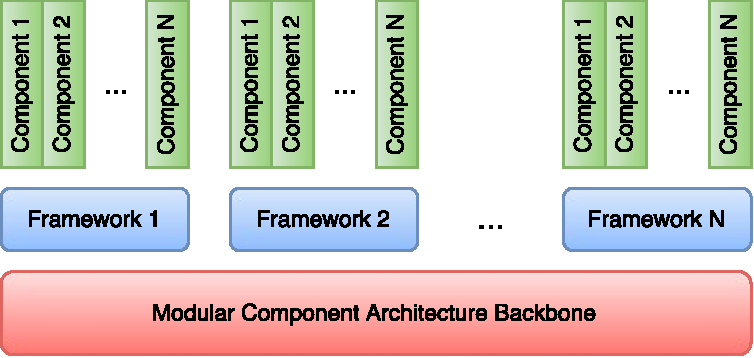
\includegraphics[scale=0.8]{img/cap3-mca.pdf}}
		\caption[Open MPI: Modular Component Architecture]{The conceptual diagram of Modular Component Architecture
                 implemented in Open MPI}
		\label{fig:cap3a-mca}
\end{figure}

\subsection{Execution Flow and Communication Layers}

\begin{figure}[t]
		\centerline 
{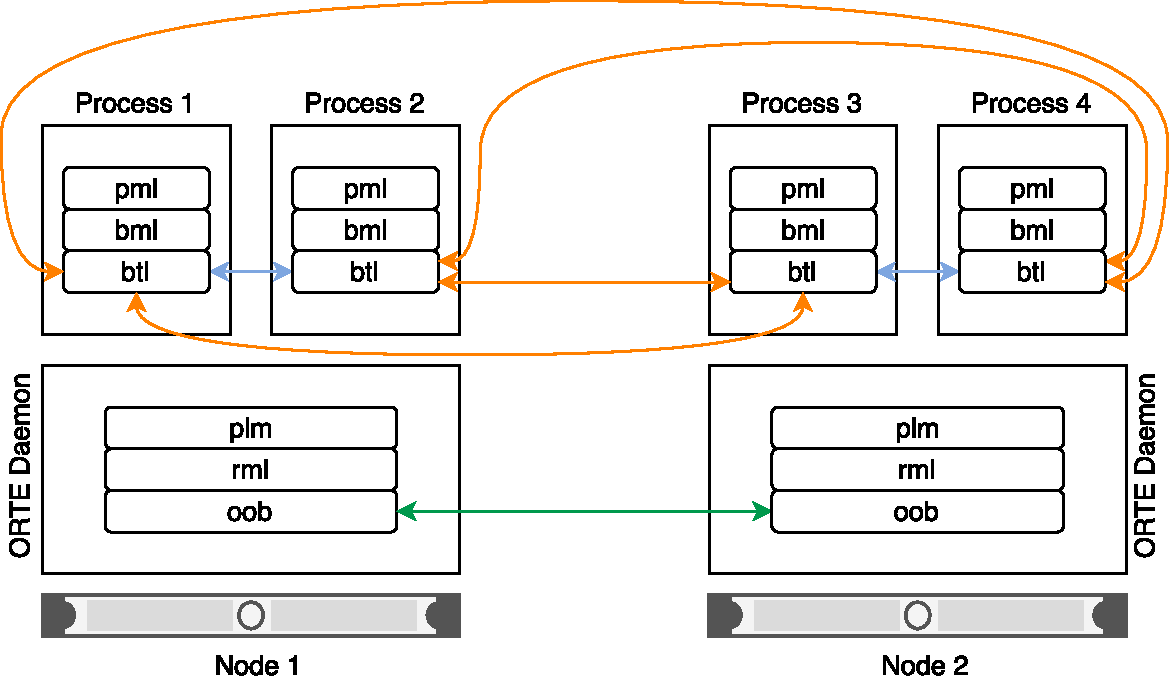
\includegraphics[scale=0.6]{img/cap3-networkdiagram.pdf}}
		\caption[Open MPI: Network connections]{Network diagram. The orange channels represent the inter-node
                 application-level communications, the cyan channels represent
                 the intra-node application-level communications, and the green
                 one represents the \texttt{orted}-level communications.}
		\label{fig:cap3-networkdiagram}
\end{figure}
After the execution of \texttt{mpirun} the HNP interrogates the
\textbf{Resource Allocator Subsystems} (\texttt{ras}) to get the list of
available nodes.
Depending on which RAS component is active, it may contact a resource manager
or perform other actions, like reading the node list from the host file (default
action if no resource manager specified). How the interaction with resource
managers works is described in the next Section \ref{sec:ompi-rm}.

The \textbf{Process Lifetime Manager} (\texttt{plm}) is subsequently in charge 
of spawning
the \emph{ORTE daemons} on the other nodes specified by the list provided by the RAS.
The PLM maintains also the communication between the various instances of
\emph{ORTE daemons} at high-level, i.e. it decodes the messages and dispatches them to
the framework in charge of handle it. The \texttt{plm} framework implementation can delegate the process spawning the
resource manager. The default selected
component - and the component used in this work - is the well known 
\textbf{Secure SHell (SSH)}.
The \texttt{orted} commands are executed in the other nodes directly via
\texttt{ssh} calls.

Subsequently to the spawning of \emph{ORTE daemons}, the coordination of the execution
takes place distributing a series of messages (having a semantic like "start X
processes on node Y")
performed at high-level by the \texttt{plm}. The \texttt{plm} entrust on two
\emph{ORTE} stacked layers, that are in charge of managing the low-level
communication: \textbf{Run-Time Messaging Layer} (\texttt{rml}) and
\textbf{Out Of Band} (\texttt{oob}). The latter manages the low-level byte
exchanges that is usually performed via a TCP/IP network.

Specularly, the application-level messaging is managed by \emph{OMPI} subsystems:
\begin{itemize}
\item \textbf{P2P Management Layer} (\texttt{pml}) catches MPI calls and manages
      fragmentation/reassembly of high-level messages;
\item \textbf{BTL Management Layer} (\texttt{bml}) provides the routing to the
      correct and optimal network device;
\item \textbf{Byte Transfer Layer} (\texttt{btl}) low-level layer in charge of
      perform system calls (e.g. socket). The current available implementations
      are: Transmission Control Protocol (TCP), InfiniBand, Portals 4,
      User-Level Generic Network Interface (uGNI), Ultra low latency Ethernet
      (usNIC).
      For intra-machine communications there are also available shared memory,    
      Intel Symmetric Communications Interface,  Vader.
\end{itemize}



The described communication architecture is summarized in Figure
\ref{fig:cap3-networkdiagram}.

\subsubsection{Input/Output}
The standard input (\texttt{stdin}), standard output (\texttt{stdout}) and
standard error\linebreak (\texttt{stderr}) of the application are
exchanged via a framework called \textbf{I/O Forwarding} (\texttt{iof}).
Particularly, each process of the application may send bytes over \texttt{stdout}
or \texttt{stderr} and may receive bytes on \texttt{stdin}. The
\texttt{iof} framework is in charge of distributing these streams across different
nodes, usually \texttt{stdout}/\texttt{stderr} towards HNP and \texttt{stdin} 
from HNP to remote daemons. This framework, like \texttt{plm}, is on top of
\texttt{rml} and \texttt{oob} layers.

When a \emph{ORTE daemon} receives \texttt{stdin} data from \texttt{iof}, it dispatches
the data to its children via a previously opened pipe\footnote{A pipe is an
unidirectional data channel used for inter-processes communication in Linux}. Vice
versa, when the \emph{ORTE daemon} receives data on pipes dedicated to \texttt{stdout}
and \texttt{stderr} it forwards the data to HNP via \texttt{iof}.

\subsection{Event Management}
The internal Open MPI events are managed by the \emph{OPAL} framework
\texttt{event}. This framework is in turn based on \textbf{libevent}
\cite{provos2003libevent}, a cross-platform event notification library.
Every component may delegate to the \texttt{event} framework the check for an
event. When the event happens, the \texttt{event} framework executes the
callback function provided.
Open MPI by default executes on a single-thread, both the \emph{ORTE} and the
\emph{OMPI} subsystems. Therefore, all functions have to execute their code and
terminate quickly in order to give back the control to the event manager
routine.

By default Open MPI adopts an \textbf{aggressive mode}: the event manager does
not voluntarily yield the processor, but only if the operating system scheduler
preempts it. Instead, if it is waiting for a specific event (like a message
coming from a socket) it keeps spinning in order to check the event firing. This
technique may help in order to reduce the \emph{reaction time}, avoiding the
context-switch overheads.

\subsection{Auxiliary Executables}
Open MPI has several executables in addition to the commands required by the
MPI standard (\texttt{mpicc}, \texttt{mpiexec}, etc.). Each executable is
linked with \emph{ORTE}, \emph{OMPI} and/or \emph{OPAL} depending on the needed
functions and the commands usually communicate with the running instances of
\emph{ORTE daemon} in order to retrieve information or perform actions.
The list and the description of available commands is presented in Appendix
\ref{app:ompicommands}.

\section{Open MPI resource management}
\label{sec:ompi-rm}
The Open MPI framework that provides resource management is the \textbf{Resource
Allocator Subsystem} (\texttt{ras}). The implementations correspond to the 
supported resource managers presented in Table \ref{tab:rmopenmpi} plus the
implementation for reading the node list from a file.
Each \texttt{ras} component has to expose four functions (in addition to the
usual functions required by MCA):
\begin{itemize}
\item \texttt{init}: a procedure called during the startup to initialize the
                     component;
\item \texttt{allocate}: it receives the job and it has to fill a list of nodes.
                         It is in charge to contact the resource manager in
                         order to request the node list and how many resources
						 available for each node;
\item \texttt{deallocate}: it receives the job that will be deallocated from the
                           nodes. Currently, all \texttt{ras} components do not
                           implement this function;

\item \texttt{finalize}: a procedure called during the shutdown to clean the
                         component and other finalization actions.

\end{itemize}

The components are called only during the setup of MPI applications, if they
do not set other events. Multiple approaches are possible, e.g. \emph{Torque}
component analyzes the environment variables or \emph{SLURM} component
tries to contact the resource manager via socket.

\section{CRIU architecture}
\textbf{Checkpoint/Restore in Userspace} - abbreviated in \textbf{CRIU} -
\cite{CRIU} is a software that exploits the recent configuration entry
\texttt{CONFIG\_CHECKPOINT\_RESTORE} in Linux.

The open source software is developed by a community mostly made of Virtuozzo
developers - a company located in Russia born from a spin-off of Parallels.

It provides several features, from the basic Checkpoint/Restart functionality
to live
migration. The services are provided through three different interfaces:
\emph{Command Line Interface} (via the \texttt{criu} command),
\emph{Remote Procedure Call} (using the Google Protocol Buffers), and the
C \emph{Application Program Interface}.

The CRIU checkpoint is invoked using the CLI interface with the following
command:

\inlinecommand{\$ criu dump -D <directory> -t <pid>}

The \texttt{-D <directory>} parameter indicates the path where the image
will be saved. The \texttt{-t <pid>} parameter indicates the PID of the
process to checkpoint. CRIU checkpoints also all the children of the specified
process. The image is saved in the provided directory, in form of several files
that can be categorized as follows:
\begin{itemize}
\item \textbf{Inventory files}: they contain the general information about the
      image, e.g. version number, system general information, etc.
\item \textbf{Image files}: the regular files that represent the process
      status. The most important are the memory dump files, that contain the 
      pages correspond to the memory content of
      the process, both private and shared. Other files contain the open file
      descriptors, the address
      space information, time states, the task credential, the mountpoints
      list, etc. 
\item \textbf{Auxiliary files}: they keep statistics and other non-essential
      information; they do not include any process data.
\end{itemize}

Similarly, the CRIU restart is performed using the CLI interface with the following command:

\inlinecommand{\$ criu restore -D <directory>}


\subsection{Linux Kernel Configuration}
The \texttt{CONFIG\_CHECKPOINT\_RESTORE} is a kernel configuration entry present
in Linux starting from version 3.11. This configuration enables additional
kernel features in order to enable Checkpoint/Restart actions in
user-space. In particular, it introduces:
\begin{itemize}

\item Some additional flags for the \texttt{prctl} system call.
      This system call allows
      the user to perform some actions on the process kernel descriptor.
      For example it is possible to change the behavior after a floating
      point exception and to request a signal send when the parent process
      terminates.
      Checkpoint/Restart requires
      to modify certain kernel memory map descriptor fields in order to restart
      correctly the process, e.g. the start address of the stack and the data
      segment size.

\item Additional \texttt{/proc} filesystem entries, again in order to ensure
      a correct restore:

\begin{itemize}

\item \texttt{/proc/[pid]/map\_files/}: this directory contains the
      \textbf{memory-mapped} files, i.e. segments of virtual memory that have
      been assigned to particular file descriptors via \texttt{mmap} system
      call.

\item \texttt{/proc/[pid]/timers}: this file provides the list of POSIX timers
      enabled for the process.

\end{itemize}

\item The \texttt{/proc/sys/kernel/ns\_last\_pid} file: it enables a privileged
      user to change the kernel internal counter used to select the next
      Process IDentifier (PID).

\end{itemize}


\subsection{The Execution Flow}

\begin{figure}[t]
    \centerline 
{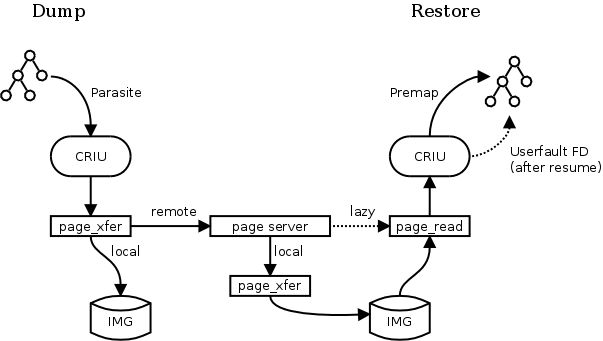
\includegraphics[scale=0.4]{img/cap3-criumemoryflow.png}}
    \caption[CRIU: Checkpoint/Restart flow diagram]{The flow diagram of the Checkpoint (Dump) and Restart (Restore)
    phases of CRIU. (Authors: CRIU Developer.
    Republishing permitted under GNU FDL 1.3) }
    \label{fig:cap3-criuexec}
\end{figure}

The flow diagram of CRIU execution is depicted in Figure
\ref{fig:cap3-criuexec}. The \emph{page server} is a CRIU component
that enables the transfer of the image to a centralized server or
to another machine. It is not currently considered for this work and we omit
other details.

Initially, a \textbf{parasite code} - built in \emph{Position-independent code
format (PIC)} - is injected into the \emph{victim} application via the
\texttt{ptrace} tool.
The \emph{parasite code} starts a daemon that will receive CRIU 
internal commands,
preparing the application for the checkpoint. The most important purpose of
this code is to save the execution context of the victim (registers,  etc.).
Subsequently, the full images of the victim process and its children are
transfered into the disk, ready to be restored. 

However, since the \emph{parasite code} is a very limited code - it cannot be
linked to any library due to the \emph{PIC} nature - some actions are executed
directly by CRIU process. The corresponding restore phase is called
\emph{Restorer context}. The data managed outside the \emph{parasite code} is:
\begin{itemize}
\item the memory content
\item all the timers information
\item the credentials (permissions, \texttt{chroot}, etc.)
\item the threads information
\end{itemize}

Before restarting the processes, the
\texttt{/proc/sys/kernel/ns\_last\_pid} has
to be set with the number immediately before the PID of the process we want to
restart, providing the file is locked exclusively.
Obviously, that PID and the PIDs of its children must be available
in the system, otherwise the process restart is not possible\footnote{This 
is a strong limitation for migration, but it will be addressed in the next
Chapter.}.

It is possible to summarize the checkpoint phases in:
\begin{enumerate}
\item Inject code in the processes tree;
\item Collect processes resources and save it;
\item Cleanup: kill the application or remote the injected code to continue 
execution.
\end{enumerate}
Specularly the restore phases perform the following actions:
\begin{enumerate}
\item Resolve shared resources in order to avoid to duplicate shared memory
region;
\item Change the PID kernel counter and fork the processes tree;
\item Restore the processes resources;
\item Restore the processes context;
\item Restore the last information (timers, threads, etc.).
\end{enumerate}

\subsection{Advantages over other C/R tools}
The first advantage is the high number currently supported architectures
compared to other C/R tools:
\begin{itemize}
\item x86
\item x86\_64
\item ARM
\item AArch64
\item PPC64le
\end{itemize}
Part of CRIU code - in particular the \textbf{parasite code} - is 
strongly architecture dependent. Apart that code, CRIU relies on
machine-independent Linux system calls.

The second, but probably the most important advantage of CRIU compared with other
C/R tools, is the
ability to run completely in user-space, even if it requires the \texttt{root}
user  permissions. Removing the limitation of administrative privileges is an
on-going development. Running in user-space instead of kernel-space
presents several advantages, among which it is possible to find: better
maintainability and portability, less security vulnerabilities
and safety risks.

The third main reason that leads us to select CRIU, is the very active
development community, that provides not only bug fixing, but also new features,
with monthly cadence releases. Some communities that developed other tools are
no more active, like BCLR.




